%! Author = MR.co
%! Date = 11/6/2022

% Preamble
\documentclass[11pt]{article}

% Packages
\usepackage{amsmath}
\usepackage{amsfonts}
\usepackage{amssymb}
\usepackage{geometry}
\usepackage{tikz}
\usepackage{float}
\usepackage{enumitem}
\usetikzlibrary{automata, arrows.meta, positioning,shapes}

\makeatletter
\newcommand{\leqnomode}{\tagsleft@true}
\newcommand{\reqnomode}{\tagsleft@false}
\makeatother

\newcommand{\abs}[1]{\vert #1\vert}
\newcommand{\tab}[1][30pt]{\hspace*{#1}}
\newcommand{\bracket}[1]{\biggl[#1\biggr]}

\newcommand{\infrule}[2]{&#1 &&\textup{#2}}
\newcommand{\subrule}{\tab[20pt]\vert\ }
\newcommand{\subinfrule}[2]{&\subrule #1 &&\textup{#2}}

\author{Ali Abbasi - 98105879}
\title{Automata Homework 1}
%\date{}

% Document
\begin{document}
\maketitle
\section{Logic, Reasoning, Induction}
\subsection{}
\subsubsection{}
\begin{align*}
p \to (q \lor r) &\equiv \neg p \lor (q \lor r)\\
&\equiv (\neg p \lor q) \lor r\\
& \equiv \neg (p \land \neg q) \lor r\\
&\equiv
(p \land \neg q) \to r
\end{align*}

\subsubsection{}
\begin{align*}
\neg (p \lor q) \lor (\neg p \land q) \lor
&\equiv (\neg p \land \neg q) \lor (\neg p \land q) \lor (p \land q)\tag{De Morgan}\\
&\equiv \biggl[\neg p \land (\neg q \lor q)\biggr] \lor (p \land q) \tag{Distributive}\\
&\equiv \bigl[\neg p \land T \bigr] \lor (p \land q)\\
&\equiv \neg p \lor (p \land q)\\
&\equiv (\neg p \lor p) \land (\neg p \lor q) \tag{Distributive}\\
&\equiv T \land (\neg p \lor q)\\
&\equiv \neg p \lor q\\
&\equiv \neg (p \land \neg q) \tag{De Morgan}
\end{align*}

\subsection{}
We are going to prove these statements both with contradiction and inference rules:
\subsubsection{}
\begin{align}
(p\to q) \implies (\neg q \to \neg p)
\end{align}
Proof with contradiction:
\begin{align*}
(p\to q) \land \neg (\neg q \to \neg p) &\equiv (\neg p \lor q) \land \neg (q \lor \neg p)\\
& \equiv (\neg p \lor q) \land (\neg q \land p)\\
& \equiv \neg q \land p \land (\neg p \lor q) \tag{reorder}\\
& \equiv \neg q \land \biggl[(p \land \neg p) \lor (p \land q)\biggr] \tag{Distributive}\\
& \equiv \neg q \land \biggl[F \lor (p \land q)\biggr]\\
& \equiv \neg q \land (p \land q)\\
& \equiv p \land (\neg q \land q) \tag{Associative}\\
& \equiv p \land F\\
& \equiv F
\end{align*}

Thus we have a contradiction.

Proof with inference rules:
\begin{subequations}
\leqnomode
\renewcommand{\theequation}{\arabic{equation}}
\begin{align}
&\neg q &&\textup{Assumption}\\
&\subrule p \to q &&\textup{Premise}\\
&\subrule \neg p &&\textup{Modus Tollens: 1, 2}\\
&\neg q \to \neg p &&\textup{$\to$ introduction: 1-3}
\end{align}
\end{subequations}

\subsubsection{}
Porof by contradiction:
\begin{equation}
\biggl[(p\to q) \land (p \to \neg q)\biggr] \implies \neg p
\end{equation}
\begin{align*}
\biggl[(p\to q) \land (p \to \neg q)\biggr] \land \neg(\neg p) &\equiv \biggl[(\neg p \lor q) \land (\neg p \lor \neg q)\biggr] \land p\\
& \equiv \biggl[\neg p \lor (q \land \neg q)\biggr] \land p\\
& \equiv \biggl[\neg p \lor F\biggr] \land p\\
& \equiv \neg p \land p\\
& \equiv F \tag*{$\therefore$ Contradiction}
\end{align*}
Proof with inference rules:
\begin{subequations}
\leqnomode
\renewcommand{\theequation}{\arabic{equation}}
\begin{align}
&p&&\textup{Assumption}\\
&\subrule p\to q &&\textup{Premise}\\
&\subrule  q && \textup{Modus Ponens: 1, 2}\\
&\subrule p \to \neg q&&\textup{Premise}\\
&\subrule \neg p &&\textup{Modus Tollens: 3, 4}\\
&\subrule  \bot &&\textup{$\neg$ elimination: 1, 5}\\
&\neg p &&\textup{$\neg$ introduction: 1-6}
\end{align}
\end{subequations}
(\(\bot\) means contradiction).\\
Note that we've used \(p\to q\) and \(p\to \neg q\) as premises for simplicity.
If we don't consider them our direct premises, then we can use Simplification rule on \((p\to q) \land (p\to \neg q)\) to get to them .

\subsubsection{}
Proof by contradiction:
\begin{equation}
\bracket{(p\lor q) \land (\neg p \lor r)} \implies (q \lor r)
\end{equation}
\begin{align*}
\bracket{(p\lor q) \land (\neg p \lor r)} \land \neg (q \lor r)
&\equiv \bracket{(p\lor q) \land (\neg p \lor r)} \land  (\neg q \land \neg r)
\\ &\equiv \bracket{(p \land \neg q) \lor (q \land \neg q)} \land \bracket{(\neg p \land \neg r) \lor (r \land \neg r)} \tag{Distributive law $\times 2$}
\\ &\equiv \bracket{(p \land \neg q) \lor F} \land \bracket{(\neg p \land \neg r) \lor F}
\\ &\equiv (p \land \neg q) \land (\neg p \land \neg r)
\\ &\equiv \neg q \land \neg r \land (p \land \neg p)
\\ &\equiv \neg q \land \neg r \land F
\\ &\equiv F  \tag*{$\therefore$ Contradiction}
\end{align*}
Proof with inference rules:
\begin{subequations}
\leqnomode
\renewcommand{\theequation}{\arabic{equation}}
\begin{align}
\infrule{\neg(q\lor r)}{Assumption}\\
\infrule{\subrule \neg q \land \neg r}{De Morgan: 1}\\
\infrule{\subrule \neg q}{Simplification: 2}\\
\infrule{\subrule p \lor q}{Premise}\\
\infrule{\subrule p}{Disjunctive Syllogism: 3, 4}\\
\infrule{\subrule \neg p \lor r}{Premise}\\
\infrule{\subrule \neg r}{Simplification: 2}\\
\infrule{\subrule \neg p}{Disjunctive Syllogism: 6, 7}\\
\infrule{\subrule \bot}{$\neg$ elimination: 5, 8}\\
\infrule{\neg \neg (q \lor r)}{$\neg$ introduction:1-9}\\
\infrule{q \lor r}{$\neg \neg$ elimination}
\end{align}
\end{subequations}

\subsection{}
\subsubsection{}
If you write a truth table for both sides, you'll see that this equivalence does not hold.
But rather we can only derive the following statement and we are going to prove that instead.
\begin{align}
(p \to r_1) \land (r_1 \to r_2) \land \ldots \land (r_n \to q) \implies p \to q
\end{align}
It is easily proved using induction.\\
\textbf{Base Case:} 
\begin{align}
    (p \to r_1) \land (r_1 \to q) \implies p \to q
\end{align}
\begin{subequations}
    \leqnomode
    \renewcommand{\theequation}{\arabic{equation}}
    \begin{align}
    \infrule{p}{Assumption}\\
    \subinfrule{p \to r_1}{Premise}\\
    \subinfrule{r_1}{Modus Ponens: 1, 2}\\
    \subinfrule{r_1 \to q}{Premise}\\
    \subinfrule{q}{Modus Ponens: 3, 4}\\
    \infrule{p \to q}{$\to$ introduction: 1-5}
    \end{align}
\end{subequations}
\textbf{Induction Hypothesis:} Let's assume for $n=k$ this equivalence holds. Then:
\begin{align}
    (p \to r_1) \land (r_1 \to r_2) \land \ldots \land (r_k \to z) \implies p \to z
\end{align}
\textbf{Induction Step:}
We can show that it also holds for $n=k+1$.
\begin{subequations}
    \leqnomode
    \renewcommand{\theequation}{\arabic{equation}}
    \begin{align}
    \infrule{(p \to r_1) \land (r_1 \to r_2) \land \ldots \land (r_{k+1} \to q)}{Premise}\\
    \infrule{(p \to r_1) \land (r_1 \to r_2) \land \ldots \land (r_{k} \to r_{k+1})}{Simplification: 1}\\
    \infrule{p \to r_{k+1}}{Induction Hypothesis: 2}\\
    \infrule{r_{k+1} \to q}{Simplification: 1}\\
    \infrule{p}{Assumption}\\
    \subinfrule{r_{k+1}}{Modus Ponens: 3, 5}\\
    \subinfrule{q}{Modus Ponens: 4, 6}\\
    \infrule{p \to q}{$\to$ introduction:}
    \end{align}
\end{subequations}
\subsubsection{}
We prove this equivalence with induction.\\
\textbf{Base Case:} for $n=1$ it's obvious:
\begin{gather*}
p = r_1\\
p \to q \equiv r_1 \to q
\end{gather*}
\textbf{Induction Hypothesis:} Let's assume for $n=k$ this equivalence holds:
\begin{gather*}
    p_1 = r_1 \lor \ldots \lor r_k\\
    p_1 \to q \equiv (r_1\to q) \land \ldots \land (r_k\to q)
\end{gather*}
\textbf{Induction Step:} Now we now show that it holds for $n=k+1$ as well:
\begin{gather*}
p = \underbrace{r_1 \lor \ldots \lor r_k}_{p_1} \lor \underbrace{r_{k+1}}_{p_2} = p_1 \lor p_2\\
\end{gather*}
\begin{align*}
(r_1\to q) \land \ldots \land (r_k\to q) \land (r_{k+1}\to q)
&\equiv (p_1 \to q) \land (r_{k+1}\to q) \tag{Induction Hypothesis}
\\ &\equiv (p_1 \to q) \land (p_2\to q)
\\ &\equiv (\neg p_1 \lor q) \land (\neg p_2 \lor q)
\\ &\equiv (\neg p_1 \land \neg p_2) \lor q \tag{Distributive law}
\\ &\equiv \neg (p_1 \lor p_2) \lor q \tag{De Morgan}
\\ &\equiv \neg p \lor q
\\ &\equiv p \to q \tab[5pt] \therefore
\end{align*}

\section{Properties of sets, recursive definitions, countability and uncountability}
\subsection{}
Yes it is a equivalence relation:
\begin{itemize}
\item \textbf{Reflexive:} \(\forall x \in L\) we define \(u\) and \(v\) as: \(u = x, v=\epsilon\).
Therefore \(x = uv = vu \implies xRx\).
\item \textbf{Symmetric:} It's obvious! (you only need to swap \(u\) and \(v\) values).
\item \textbf{Transitive:} Assume \(\abs{x} = n=i+j\) and \(x\) is split into \(u\) and \(v\) at index \(i\) (i.e., \(\abs{u}=i, \abs{v}=j\))
and \(y=vu\).
And we know \(yRz\); i.e., if we split y at some index and swap the resulting substrings, we get \(z\).
There is three possibilities for index at which \(y\) is split.
If \(y\) is split at index \(k=j\), then \(x=z\) and \(xRz\) by reflexiveness.
If y is split at \(0\leq k < j\), then one can rewrite \(x, y\), and \(z\) as follow:
\(y=abu, x=\underbrace{ua}_{u\prime}\underbrace{b}_{v\prime}, z=\underbrace{b}_{v\prime}\underbrace{ua}_{u\prime}\) (where \(\abs{a} = k\)) and as you can see, you can convert \(x\) to \(z\) and vice versa, by swapping \(u\prime\) and \(v\prime\).
Thus \(xRz\).
You can show same thing in the case where split is done at index \(j \leq k < n\) with a similar procedure.
Hence \(R\) is transitive.
\end{itemize}
\subsection{}
\subsubsection{}
We name the mentioned set \(S\) and define \(S\) recursively:
\begin{enumerate}[label=\textnormal{(\arabic*)}]
    \item \(a \in S\)
    \item \(\forall x, y \in S: \ x+y \in S\)
    \item \(\forall x, y \in S: \ x\times y \in S\)
    \item \(\forall x \in S: \ (x) \in S\)
\end{enumerate}
Now we prove string \((a + a \times (a + a))\) belongs to \(S\) by constructing it step by step with the above rules:
\begin{enumerate}
\item \(\xrightarrow{(1)} a \in S\)
\item \(\xrightarrow{1, (2)} a + a \in S\)
\item \(\xrightarrow{2, (4)} (a + a) \in S\)
\item \(\xrightarrow{1, 3, (3)} a\times (a + a) \in S\) 
\item \(\xrightarrow{1, 4, (2)} a + a\times (a + a) \in S\) 
\item \(\xrightarrow{5, (4)} (a + a\times (a + a)) \in S\) 
\end{enumerate}
(Numbers in parenthesis refer to rules defined above).
\subsubsection{}
We name the mentioned set \(S\) and define \(S\) recursively:
\begin{enumerate}[label=\textnormal{(\arabic*)}]
    \item \(\epsilon \in S\)
    \item \(\forall x \in S: \ (x) \in S\)
    \item \(\forall x, y \in S: \ xy \in S\)
\end{enumerate}
Now we prove \(()(()) \in S\) by constructing it step by step:
\begin{enumerate}
    \item \(\xrightarrow{(1)} \epsilon \in S\)
    \item \(\xrightarrow{1, (2)} () \in S\)
    \item \(\xrightarrow{2, (2)} (()) \in S\)
    \item \(\xrightarrow{3, 2, (3)} (())() \in S\)
\end{enumerate}
\subsection{}
We assume disks in \(A\) do not have any overlap with each other. \\
You can find a point \((x, y)\) at every disk such that \(x, y \in \mathbb{Q}\) (because every disk covers a range of real number in both axes, and you can find a rational number in every real range).
We map every disk to one of its points with rational coordinates and
since disks are disjoint, this mapping would be a one-to-one function.
Thus we have mapped the set \(A\) to a subset of \(\mathbb{Q}^2\) and as we know, \(\mathbb{Q}\) and \(\mathbb{Q}^2\) are both countable sets.
Thus \(\abs{A} \leq \abs{\mathbb{Q}^2}\) and \(A\) is countable.

\subsection{}
In this case, \(A\) can be uncountable.
Consider only set of circles with their center at origin and a radius of \(r \in (0, 1]\).
There can be as many (non-intersecting) circles in this set as cardinality of \((0, 1]\) which we know is higher than \(\abs{J}\) hence it is not countable.

\section{Basics of Automata}
\subsection{}
We add a new state to the automata (\(s\)) and want to determine new transition function's output for state \(q\) and letter \(t\) (i.e., \(\delta^\prime(q, t)\)).
There is three cases:
\begin{enumerate}
    \item If \(q\) is an accepting state in \(A\) and there is some state which goes to \(q\) with \(t\), then in the new automata, \(\delta^\prime(q, t) = s\).
    For example, state \(4\) is an accepting state and state \(2\) goes to \(4\) by receiving letter \(b\).
    So in the new automata, \(\delta^\prime(4, b) = s\).

    \item If \(q\) is not in accepting states and if all states that have an edge to \(q\), go to \(q\) with all receiving letters (except \(t\)), then \(\delta^\prime(q, t) = s\).
    For example, \(\delta^\prime(2, a) = s\). Because all of  in-neighbors (neighbors with an incoming edge) of \(2\) (only \(1\)) are connected to \(2\) with \(\Sigma - \{a\} = b\).

    \item If it's non of above rules applied, \(\delta^\prime\) acts similar to \(\delta\).
\end{enumerate}
By applying these rules, the new state machine would be as follow:

\begin{figure}[H]
    \centering
    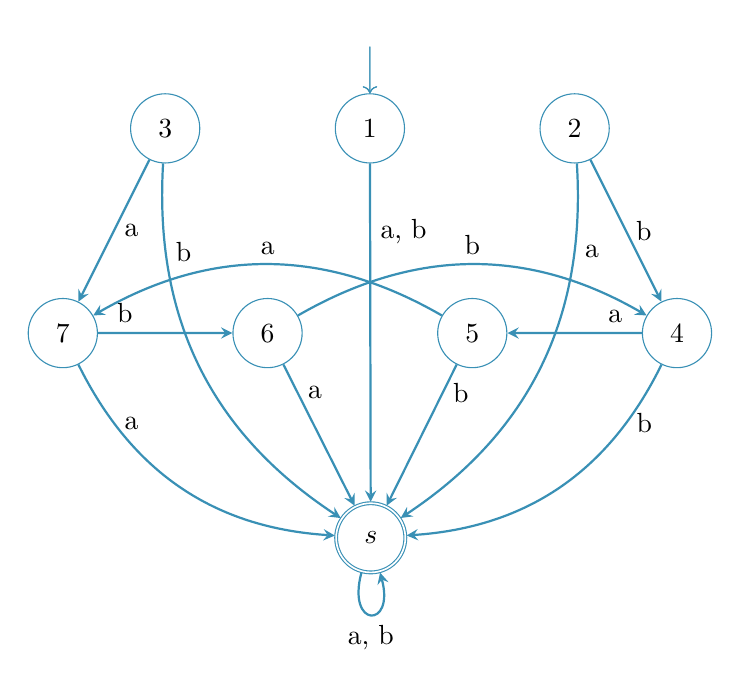
\begin{tikzpicture} [draw=cyan!70!black,
    node distance = 3cm,
    on grid,
    right,
    every loop/.style={stealth-}, scale=1.3]

\node (s) [state, accepting,] {$s$};

\node (q1) [state, initial, initial text = {}, initial above] at (0, 4) {$1$};

\node (q2) [state] at (2, 4) {$2$};

\node (q3) [state] at (-2, 4) {$3$};

\node (q4) [state] at (3, 2) {$4$};

\node (q7) [state] at (-3, 2) {$7$};

\node (q5) [state] at (1, 2) {$5$};

\node (q6) [state] at (-1, 2) {$6$};

% Arrows
\path [-stealth, thick]
(s) edge [loop below] node {a, b} (s)
(q1) edge [pos=0.2] node {a, b} (s)
(q2) edge [bend left, pos=0.2] node {a} (s)
(q4) edge [bend left, pos=0.2] node {b} (s)
(q5) edge [pos=0.2] node {b} (s)
(q3) edge [bend right, pos=0.2] node {b} (s)
(q6) edge [pos=0.2] node {a} (s)
(q7) edge [bend right, pos=0.2] node {a} (s)
(q2) edge node {b} (q4)
(q3) edge node {a} (q7)
(q4) edge [above, pos=0.2] node {a} (q5)
(q7) edge [above, pos=0.2] node {b} (q6)
(q5) edge [above, bend right] node {a} (q7)
(q6) edge [above, bend left] node {b} (q4);
\end{tikzpicture}
    \caption{New automata (\(A^\prime\))}
    \label{fig:3.1dfa}
\end{figure}

Note that rule number 2 is vacuously true for states \(1\) and \(s\); because they have no in-neighbors in transition function \( \delta \).
So resulting state machine would be the same as a state machine with only states \(1\) and \(s\) with \(\delta^\prime(1, a) = s\), \(\delta^\prime(1, b) = s\), \(\delta^\prime(s, a) = s\), \(\delta^\prime(s, b) = s\) as its only edges.
\end{document}


    

